\documentclass[conference]{IEEEtran}
\IEEEoverridecommandlockouts
\usepackage{cite}
\usepackage{balance}
\usepackage{amsmath,amssymb,amsfonts}
\usepackage{graphicx}
\usepackage{textcomp}
\usepackage{xcolor}
\usepackage{booktabs}
\usepackage{algorithm}
\usepackage{algorithmic}
\usepackage{tikz}
\usetikzlibrary{positioning,arrows.meta,fit,calc}
\usepackage[hidelinks]{hyperref}
\input{nums.tex}

\begin{document}

\title{Runtime Assurance for Sampling-Based Optimizers\\
in Flood Re-Planning: Exact Verification and\\
Certified Escalation}

%<AUTHORS>
\author{
\IEEEauthorblockN{Nandhakumar T}
\IEEEauthorblockA{\textit{Department of Information Technology}\\
\textit{Sona College of Technology}\\
Salem, Tamil Nadu, India\\
nandhakumartm93@gmail.com}
\and
\IEEEauthorblockN{Balakarthikeyan B S}
\IEEEauthorblockA{\textit{Department of Artificial Intelligence and Data Science}\\
\textit{Sona College of Technology}\\
Salem, Tamil Nadu, India\\
balasan2626@gmail.com}
\and
\IEEEauthorblockN{Gowthaman J}
\IEEEauthorblockA{\textit{Department of Artificial Intelligence and Data Science}\\
\textit{Sona College of Technology}\\
Salem, Tamil Nadu, India\\
gowthamanjanadhran@gmail.com}
\and
\IEEEauthorblockN{Abhishek S}
\IEEEauthorblockA{\textit{Department of Artificial Intelligence and Data Science}\\
\textit{Sona College of Technology}\\
Salem, Tamil Nadu, India\\
abisheksengodan18@gmail.com}
}
%</AUTHORS>

\maketitle

\begin{abstract}
Quantum and annealing-based optimizers are proposed for disaster logistics, yet they return samples with no guarantee of validity, and the penalty encodings they need are often inexact. We study how a re-planning loop can use such samplers safely when evacuation groups must be reassigned to shelters as roads close and shelters fail. The loop verifies every sample exactly against the current state, falls back to a greedy rule, and, before handing a case to a human, asks an exact mixed-integer program (MILP) whether any valid plan exists. On \TwinEvents{} re-planning events of a flood digital twin (12 binary variables), dispatching the most frequent sample unchecked would have sent an invalid plan in \TwinRawFeasQ\% of draws on solvable events for the Quantum Approximate Optimization Algorithm (QAOA) and \TwinRawFeasSA\% for simulated annealing (\TwinRawQ\% and \TwinRawSA\% counting events with no valid plan). Taking the lowest-energy sample, or the lowest-energy sample that satisfies every penalty, still dispatched an invalid plan in \BaseLowQSol\% and \BasePfQSol\% of solvable QAOA draws, because the pairwise capacity penalty cannot see overloads by three groups; the verified loop dispatched none. On \CityN{} instances built on OpenStreetMap road networks of six Indian cities with up to \CityMaxVars{} variables, the annealer's valid-plan rate on solvable instances fell from \CitySAFoundEight\% at 8 groups to \CitySAFoundThirtyTwo\%, and an uncertified loop escalated \CityFalseEsc\% of solvable cases to a human. The MILP settled all \CityN{} instances, the slowest in \MilpSlowS~s; a \DeadlineS~s deadline would have stopped \DeadlineN{} of them without a plan or a proof, yet all had valid plans, so a solver time-out must never be read as infeasibility. At these sizes calling the MILP first was faster and always optimal, so the samplers add no value yet; the loop is the safety wrapper any future sampler needs.
\end{abstract}

\begin{IEEEkeywords}
runtime assurance, quantum optimization, simulated annealing, mixed-integer programming, evacuation planning
\end{IEEEkeywords}

\section{Introduction}
When a flood closes roads and fills shelters, the assignment of evacuation groups to shelters has to be re-made, often many times in one night. The assignment is a small constrained optimization problem, and it is a common showcase for quantum and quantum-inspired optimizers, which take it as a quadratic unconstrained binary optimization (QUBO) problem \cite{Lucas2014,Glover2019,Cadelina2024,Abbas2024}. Two properties of these tools matter more for an operations room than their speed. They return \emph{samples}, so the same call can give a different, possibly invalid answer. And the QUBO they solve encodes capacity limits with penalties, which is exact only in special cases: a sample that satisfies every penalty can still overfill a shelter.

Safety-critical engineering has a standard answer to unreliable components: run them inside a \emph{runtime-assurance} architecture, in which a simple verified controller checks or replaces the complex one \cite{Sha2001,Desai2019}, as shields do for learned policies \cite{Alshiekh2018}. Three questions arise when the complex component is a sampling optimizer. How often would its output be unsafe without the check? When no sample is valid, how does the loop know whether to try harder or to call a human? And how many samples should it draw?

We answer them for flood re-planning. Our contributions are:
\begin{enumerate}
\item A runtime-assurance loop for sampling optimizers with an exact plan verifier, a greedy fallback and a \emph{certified escalation} step that uses a mixed-integer program (MILP) to decide whether any valid plan exists (Fig.~\ref{fig:loop}).
\item A measurement on twin episodes with QAOA \cite{Farhi2014,Hadfield2019} and simulated annealing \cite{Kirkpatrick1983} of how often unverified dispatch would be unsafe, for the most frequent, the lowest-energy and the best penalty-free sample, with a classification of every unsafe sample by the rule it breaks.
\item A city-scale study on OpenStreetMap road graphs of six Indian cities, beyond the reach of enumeration, showing where samplers and uncertified loops fail, what the certificate costs, and why a solver time-out is not a proof.
\item A comparison with an exact-solver-first loop in time and plan cost, and a shot-budget bound with an adaptive budget.
\end{enumerate}
All QAOA results are classical simulations; we make no claim of quantum speed-up.

\section{Related Work}
\textit{Runtime assurance.} The Simplex architecture switches from an unverified high-performance controller to a verified safety controller when the former leaves a safe envelope \cite{Sha2001}; SOTER brings the pattern to robotics software \cite{Desai2019}, shields apply it to reinforcement learning \cite{Alshiekh2018}, and runtime verification checks executions against a specification as they happen \cite{Leucker2009}. Levels-of-automation theory argues that automation should fall as the cost of an error rises \cite{Parasuraman2000}. Our verifier is the switching logic, and the MILP plays the role of the verified controller of last resort.

\textit{Samplers as tools.} Variational quantum algorithms are hybrid loops in which a classical optimizer calls a quantum circuit \cite{McClean2016}; QAOA with constraint-preserving mixers keeps one-hot structure but still penalizes capacity \cite{Hadfield2019,WangZ2020}. Quantum annealing has been applied to disaster resource allocation \cite{Cadelina2024}, and reviews stress that practical advantage in optimization is unproven \cite{Abbas2024}. Agent frameworks let language models call tools \cite{Yao2023,Schick2023}, and runtime enforcement constrains the actions such agents may take \cite{WangH2026}; these works do not check the plans an optimizer returns.

\textit{Evacuation planning.} Shelter allocation has long been solved with integer programming \cite{Sherali1991}; modern MILP solvers such as HiGHS \cite{Huangfu2018} make exact solutions cheap at the sizes of a city district. Repairing a plan rather than re-planning from scratch reduces disruption \cite{Fox2006}.

Table~\ref{tab:pos} summarizes the gap. We found no application of runtime assurance to sampling optimizers, and the sampler studies cited here report solution quality per call; none measures what happens when a loop acts on the answer.

\begin{table}[t]
\caption{Position of this work}
\label{tab:pos}
\centering
\footnotesize
\setlength{\tabcolsep}{2.4pt}
\begin{tabular}{llll}
\toprule
Work & Unreliable part & Check & Escalation\\
\midrule
Simplex, SOTER \cite{Sha2001,Desai2019} & controller & envelope & safe controller\\
Shielding \cite{Alshiekh2018} & RL policy & automaton & blocked action\\
QUBO for disasters \cite{Cadelina2024} & annealer & -- & --\\
This work & sampler & exact verifier & MILP-certified\\
\bottomrule
\end{tabular}
\end{table}

\section{Problem and Loop}
\subsection{Assignment}
Groups $g=1,\dots,G$ of size $n_g$ are assigned to shelters $s=1,\dots,S$ with remaining seats $R_s$. With travel cost $c_{gs}$ on the best open path and a set $\mathcal F$ of forbidden pairs (no open path, failed shelter, group larger than the seats left), a plan $\mathbf x\in\{0,1\}^{G\times S}$ is valid when
\begin{multline}
V(\mathbf x)=\Big[\textstyle\sum_s x_{gs}=1\ \forall g\Big]\wedge\Big[x_{gs}=0\ \forall (g,s)\in\mathcal F\Big]\\
\wedge\Big[\textstyle\sum_g n_g x_{gs}\le R_s\ \forall s\Big],
\label{eq:valid}
\end{multline}
and the planner minimizes $\sum_{g,s}c_{gs}x_{gs}$ over valid plans. Samplers solve the QUBO with a per-group shifted cost, a one-hot penalty and a pairwise penalty $P\,x_{gs}x_{hs}$ for every two groups that together exceed $R_s$ \cite{Glover2019}. The pairwise term misses overloads by three or more groups whose pairs all fit, so a sample can satisfy every penalty and still violate (\ref{eq:valid}).

\subsection{Runtime-Assurance Loop}
Algorithm~\ref{alg:loop} gives the loop. It verifies every sample with (\ref{eq:valid}) against the state at dispatch time, keeps the cheapest valid one, falls back to a greedy rule (largest group first to its cheapest shelter with seats left), and only then asks the MILP
\begin{equation}
\min_{\mathbf x}\ \sum_{g,s}c_{gs}x_{gs}\quad\text{s.t. (\ref{eq:valid})},\ x_{gs}\in\{0,1\}.
\label{eq:milp}
\end{equation}
If (\ref{eq:milp}) is infeasible, escalation to a human is \emph{certified}: no valid plan exists. If it is feasible, the loop dispatches its plan instead of escalating. If the solver stops at its time limit, the loop escalates but marks the case \emph{uncertified}, so the officer knows that a plan may exist. A loop that escalates whenever the sampler and greedy rule fail, without asking the MILP, is the natural baseline; we call it the uncertified loop.

\begin{algorithm}[t]
\caption{Runtime-assurance re-planning at one event}
\label{alg:loop}
\begin{algorithmic}[1]
\small
\STATE draw shots in batches of $b$ until a sample passes $V$ or the budget $N$ is used
\STATE $\mathbf x\leftarrow$ cheapest sample with $V(\mathbf x)$; \textbf{if} none, $\mathbf x\leftarrow$ greedy
\IF{$V(\mathbf x)$}
\STATE dispatch $\mathbf x$
\ELSE
\STATE solve (\ref{eq:milp}) with a time limit
\STATE \textbf{if} feasible, dispatch its plan; \textbf{if} infeasible, escalate with the certificate
\STATE \textbf{if} timed out, escalate marked as uncertified
\ENDIF
\end{algorithmic}
\end{algorithm}

\begin{figure}[t]
\centering
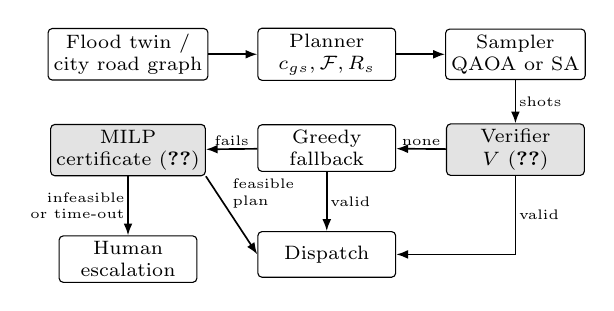
\begin{tikzpicture}[font=\scriptsize,
  box/.style={draw, rounded corners=1.5pt, align=center, minimum width=1.75cm, minimum height=0.58cm, inner sep=2pt},
  safe/.style={box, fill=gray!22},
  lab/.style={font=\tiny, inner sep=1pt},
  arr/.style={-{Latex[length=1.5mm]}, semithick}]
\node[box] (tw) {Flood twin /\\city road graph};
\node[box, right=0.62cm of tw] (pl) {Planner\\$c_{gs},\mathcal F,R_s$};
\node[box, right=0.62cm of pl] (sm) {Sampler\\QAOA or SA};
\node[safe, below=0.55cm of sm] (ve) {Verifier\\$V$ (\ref{eq:valid})};
\node[box, below=0.55cm of pl] (gr) {Greedy\\fallback};
\node[safe, below=0.55cm of tw] (mi) {MILP\\certificate (\ref{eq:milp})};
\node[box, below=0.75cm of gr] (di) {Dispatch};
\node[box, below=0.75cm of mi] (hu) {Human\\escalation};
\draw[arr] (tw) -- (pl);
\draw[arr] (pl) -- (sm);
\draw[arr] (sm) -- node[lab, right]{shots} (ve);
\draw[arr] (ve) -- node[lab, above]{none} (gr);
\draw[arr] (gr) -- node[lab, above]{fails} (mi);
\draw[arr] (gr) -- node[lab, right]{valid} (di);
\draw[arr] (ve.south) |- node[lab, pos=0.25, right]{valid} (di.east);
\draw[arr] (mi) -- node[lab, left, align=right]{infeasible\\or time-out} (hu);
\draw[arr] (mi.south east) -- node[lab, above right, pos=0.45, align=left]{feasible\\plan} (di.west);
\end{tikzpicture}
\caption{Runtime-assurance loop. Shaded blocks are exact, and the sampler is never trusted. A human is called when the MILP proves that no valid plan exists, or, flagged as uncertified, when it runs out of time.}
\label{fig:loop}
\end{figure}

\subsection{Shot Budget}
If one shot is valid with probability $q$, the chance that $N$ independent shots contain no valid plan is $(1-q)^N$, so
\begin{equation}
N\ \ge\ \frac{\ln\epsilon}{\ln(1-q)}
\label{eq:shots}
\end{equation}
shots make that chance at most $\epsilon$. Since $q$ is unknown and changes with every event, the loop draws batches of $b=\Batch$ shots and stops at the first batch with a valid sample, up to $N=\Shots$. A wrong guess of $q$ then costs shots or plan quality, while the verifier and certificate still stand behind every decision.

\section{Experimental Setup}
\textit{Twin episodes.} We replay \TwinSeeds{} seeded episodes of a flood digital twin with four groups and three shelters (12 binary variables): the initial state, closure of road R5, a shelter surge of half its capacity, a further random closure, the failure of shelter A and, as a final stress, the failure of shelter B (\TwinEvents{} re-planning events, \TwinInfeasible{} of them without any valid plan). QAOA uses a ring-XY mixer at depth 3, trained per event by COBYLA with layer-wise interpolation \cite{Zhou2020}. Simulated annealing runs on the same QUBO as 64 independent chains per call, one shot per chain, with 30 sweeps. Each event is sampled ten times with independent seeds, 64 shots per draw.

\textit{City instances.} We built \CityN{} instances on the OpenStreetMap road graphs of Delhi, Chennai, Mumbai, Kolkata, Guwahati and Patna, with the mapped zones and ten shelters per city, $G\in\{8,16,32\}$ groups (\CityMinVars--\CityMaxVars{} variables), demand of 60\% or 90\% of the seats left, and a disruption that closes the three most flood-exposed roads and fails one shelter. Travel times follow the prototype's router (flood- and traffic-weighted length at 25~km/h); capacities are building-type estimates from the city data, and group sizes are synthetic. Simulated annealing runs 64 chains of 40 sweeps per call, ten times per instance; on three instances per city, size and demand we repeated it with 400 sweeps. At this scale the annealer is the only sampler; QAOA is not simulated. All city results come from one run on a frozen copy of the city data, whose SHA-256 sums are released with the scripts. Enumeration of $10^{G}$ plans is impossible here, so the MILP is the only exact reference.

\textit{Metrics.} Unsafe dispatch: the sample a naive loop would act on violates (\ref{eq:valid}). We score three such integrations: the most frequent sample, the lowest-energy sample, and the lowest-energy sample among those with zero penalty, i.e.\ the samples that pass the encoding's own constraints. False escalation: a case escalated although (\ref{eq:milp}) has a solution. Optimality gap: excess travel cost of the dispatched plan over the MILP optimum. Times are wall-clock on a laptop running three instances in parallel. The draws of one event share its instance, so they are not independent samples of the event population.

\section{Results}
\subsection{Twin Episodes}
Table~\ref{tab:twin} gives the twin results over \TwinEvents{} events and ten draws each. \TwinText{} \StatText{}

Table~\ref{tab:trace} follows one episode with QAOA through its six events (seed \TraceSeedNo, the one in which the greedy rule did the most work). In the first two events the trained state put almost all of its probability on valid plans. After the surge it put only \TracePfTwo{} there, and after the second closure \TracePfThree{}, so the most frequent sample was invalid in every draw from then on. After the surge the verifier still picked out a rare valid sample in some draws; otherwise the greedy rule supplied the plan, and no dispatched plan cost more than \TraceGreedyGap\% above the optimum. When shelter B failed, the MILP proved that no plan existed and the loop escalated with a certificate.



\begin{table}[t]
\caption{Twin episodes: \TwinEvents{} events $\times$ 10 draws, 12 variables}
\label{tab:twin}
\centering
\footnotesize
\setlength{\tabcolsep}{2.2pt}
\begin{tabular}{lccccc}
\toprule
Sampler, budget & Unsafe & Valid & Optimal & Shots & False\\
 & if unverified & sample & dispatched & used & escal.\\
\midrule
\input{tab_twin.tex}
\bottomrule
\multicolumn{6}{l}{\scriptsize All in \% except shots. False escal.: uncertified loop; the certified loop had none.}\\
\end{tabular}
\end{table}

\begin{table}[t]
\caption{One twin episode with QAOA (seed \TraceSeedNo, 10 draws per event)}
\label{tab:trace}
\centering
\footnotesize
\setlength{\tabcolsep}{2.2pt}
\begin{tabular}{lccccc}
\toprule
Event & Plan & $P$(valid) & Top sample & Plan source & Max.\\
 & exists & of state & unsafe & (draws) & gap \%\\
\midrule
\input{tab_trace.tex}
\bottomrule
\end{tabular}
\end{table}

Table~\ref{tab:event} splits the twin results by event. \EventText{}

\begin{table}[t]
\caption{Twin results by event: unsafe if dispatched unverified, optimal under the verified loop (30 events each; \% of draws)}
\label{tab:event}
\centering
\footnotesize
\setlength{\tabcolsep}{3pt}
\begin{tabular}{lccccc}
\toprule
Event & No valid & \multicolumn{2}{c}{Unsafe} & \multicolumn{2}{c}{Optimal}\\
 & plan & QAOA & SA & QAOA & SA\\
\midrule
\input{tab_event.tex}
\bottomrule
\end{tabular}
\end{table}

\subsection{City Scale}
Table~\ref{tab:city} and Fig.~\ref{fig:city} give the city results. \CityText{}

Fig.~\ref{fig:milp} shows what the certificate costs. The median MILP time rose from \MilpMedEight~s at 80 variables to \MilpMedThirtyTwo~s at 320, so at district scale a typical certificate takes under a second; the cost lies in the rare slow instances. Resampling the solvable instances puts the false-escalation rate of the uncertified loop at \CityFalseLo--\CityFalseHi\% (95\% interval).


\begin{table}[t]
\caption{City instances on OpenStreetMap road graphs (6 cities)}
\label{tab:city}
\centering
\footnotesize
\setlength{\tabcolsep}{2.0pt}
\begin{tabular}{cccccccc}
\toprule
$G$ & vars & demand & feasible & valid & unsafe & false esc. & MILP\\
 & & & inst. & sample \% & \% & uncert. \% & s (max)\\
\midrule
\input{tab_city.tex}
\bottomrule
\multicolumn{8}{l}{\scriptsize valid: verified plan in 64 SA shots; unsafe: top sample unchecked.}\\
\multicolumn{8}{l}{\scriptsize --: none solvable. No run reached the \CityLimitS~s limit.}\\
\end{tabular}
\end{table}

\begin{figure}[t]
\centering
\includegraphics[width=\columnwidth]{fig_city.pdf}
\caption{City scale: share of calls in which the sampler produced a valid plan, and share of solvable cases an uncertified loop would escalate, against the number of groups.}
\label{fig:city}
\end{figure}

\begin{figure}[t]
\centering
\includegraphics[width=\columnwidth]{fig_milp.pdf}
\caption{Cost of the certificate: MILP solve time of every city instance (log scales, sizes jittered). The dotted line marks a \DeadlineS~s deadline; every instance above it had a valid plan.}
\label{fig:milp}
\end{figure}

Table~\ref{tab:bycity} gives the same results per city. \ByCityText{}

\begin{table}[t]
\caption{City instances by city (60 instances each; \% unless noted)}
\label{tab:bycity}
\centering
\footnotesize
\setlength{\tabcolsep}{2.4pt}
\begin{tabular}{lcccccc}
\toprule
City & Solvable & Valid & Unsafe & False esc. & Greedy & MILP s\\
 & & sample & & uncert. & found & (median)\\
\midrule
\input{tab_bycity.tex}
\bottomrule
\end{tabular}
\end{table}

\subsection{Why Unverified Samples Fail}
\label{sec:viol}
Table~\ref{tab:viol} classifies every unsafe top sample by the first rule of (\ref{eq:valid}) it breaks. \ViolText{}

\begin{table}[t]
\caption{First rule broken by the unsafe top samples (\% of unsafe samples)}
\label{tab:viol}
\centering
\footnotesize
\setlength{\tabcolsep}{2.6pt}
\begin{tabular}{lccccc}
\toprule
Sampler & Unsafe & One-hot & Forbidden & \multicolumn{2}{c}{Overload}\\
 & draws & broken & pair & penalized & penalty-free\\
\midrule
\input{tab_viol.tex}
\bottomrule
\end{tabular}
\end{table}

\subsection{Usual Practice and an Exact Solver First}
\label{sec:base}
Table~\ref{tab:base} scores the integrations that sampler studies usually rely on. \BaseText{}

\begin{table}[t]
\caption{Unsafe if dispatched unverified, by integration (\% of draws)}
\label{tab:base}
\centering
\footnotesize
\setlength{\tabcolsep}{2.2pt}
\begin{tabular}{lccccc}
\toprule
 & \multicolumn{2}{c}{Twin, QAOA} & \multicolumn{2}{c}{Twin, SA} & City, SA\\
Dispatched sample & all & solvable & all & solvable & solvable\\
\midrule
\input{tab_base.tex}
\bottomrule
\end{tabular}
\end{table}

\ExactFirstText{} \StrongText{}

\subsection{Shot Budget}
\ShotText{} By (\ref{eq:shots}), a sampler with $q=0.05$ needs 90 shots for $\epsilon=0.01$, more than the \Shots{} used here.

\section{Discussion and Limitations}
The study separates two questions that are often merged: whether a solver gives good answers, and whether a system built on it acts safely. The second holds by construction whenever every sample is verified, a classical plan is always available and the certificate finishes in time, and it holds for any sampler plugged in. The sampler decides how often the exact components have to step in. At city scale the pairwise capacity QUBO broke down and the sampler rarely contributed a valid plan, so an uncertified loop would have woken an officer for cases that a MILP solved in seconds. At every size we tested, calling the MILP first would have been faster in median time and always optimal; the samplers earned their place only as a stand-in for future hardware, and the loop is the part that would carry over to it.

The certificate has its own failure mode, the time limit. No run reached our 60~s limit, but under a \DeadlineS~s deadline \DeadlineN{} city instances would have stopped with neither plan nor proof, and all of them had plans. An implementation that reads a time-out as ``no plan'' would have escalated them with a false certificate.

The results translate into four rules for anyone wiring a sampler into an operations loop:
\begin{enumerate}
\item Verify every sample against the state at dispatch time. Even on solvable twin events the top sample was unsafe in \TwinRawFeasSA--\TwinRawFeasQ\% of draws, and the best penalty-free sample in \BasePfQSol\%; at city scale most calls were unsafe.
\item Ask an exact solver before calling a human, and call it first whenever it fits the deadline. Without it, \CityFalseEsc\% of solvable city cases reached an officer, and the greedy fallback cost a median \CityGreedyGap\% more than the optimum.
\item Set the solver limit from the decision deadline and report a time-out as unknown, never as infeasible.
\item Keep the full shot budget when plan quality matters. The adaptive budget never changed an escalation, but it lowered QAOA's rate of optimal plans from \FixedOptQ\% to \AdaptOptQ\%.
\end{enumerate}

\textit{Threats to validity.} Several design choices shape the numbers. The penalty weight $P$ is set once per instance from the cost range, as in the usual QUBO recipe \cite{Glover2019}, and was not tuned; a larger $P$ changes how often samples break the penalized rules, while the overloads that the pairwise term misses stay invisible at any weight. QAOA was trained per event with a fixed budget and simulated without noise at 12 variables, and the city study uses simulated annealing as its only sampler, so we expect a noisy hardware sampler to produce valid samples less often. The draws of one event share its instance, which is why the intervals above resample events and instances rather than draws.

The external limits are those of the data. City demand is synthetic, capacities are estimates by building type, and every city instance uses the same kind of disruption: three closed roads and one failed shelter. The MILP is exact, but the slowest 320-variable instance needed \MilpSlowS~s, and regional problems will hit any fixed limit more often. Escalation was tested for infeasibility caused by failures and closures, and no officer took part in the evaluation, so the cost of a false escalation to a real operations room is not measured here.

\section{Conclusion}
Sampling optimizers can join a flood re-planning loop safely if the loop never trusts them. An exact verifier checks every sample, a greedy rule and a MILP stand behind the sampler, and a human is called when the MILP proves that no plan exists or runs out of time, the second case flagged as uncertified. Without verification, the most frequent sample would have been unsafe in \TwinRawFeasQ\% of draws on solvable twin events for QAOA and \TwinRawFeasSA\% for annealing, and choosing the lowest-energy or the best penalty-free sample did not remove the risk, because the encoding cannot see some overloads. Without certification, the loop escalated \CityFalseEsc\% of solvable city cases. With both, no invalid plan was dispatched, and the MILP settled \CitySettled{} of \CityN{} city instances within \MilpMaxS~s. At these sizes an exact solver alone was faster and optimal, so the samplers add no value yet; we claim no quantum advantage. The results describe the checks that any such optimizer needs around it before it can act on a flood.

\section*{Acknowledgment}
The authors thank the OpenStreetMap contributors for openly available map data.
In line with the IEEE policy on AI-generated content, the authors disclose that Claude (Anthropic) was used to help edit and restructure the text of all sections and to draft the simulation, experiment and plotting scripts. All experiments use the authors' own software and fixed seeds. The authors checked every number, claim and reference and take full responsibility for the content.

\balance
\begin{thebibliography}{00}
\bibitem{Lucas2014} A. Lucas, ``Ising formulations of many NP problems,'' \textit{Front. Phys.}, vol. 2, Art. no. 5, 2014, doi: 10.3389/fphy.2014.00005.
\bibitem{Glover2019} F. Glover, G. Kochenberger, and Y. Du, ``Quantum bridge analytics I: A tutorial on formulating and using QUBO models,'' \textit{4OR}, vol. 17, no. 4, pp. 335--371, 2019, doi: 10.1007/s10288-019-00424-y.
\bibitem{Cadelina2024} A. R. Cadeli\~{n}a \textit{et al.}, ``D-Wave implementation of quantum annealing for optimal resource allocation in disaster response operation of Marikina City,'' \textit{ECTI Trans. Comput. Inf. Technol.}, vol. 18, no. 1, pp. 24--33, 2024, doi: 10.37936/ecti-cit.2024181.253577.
\bibitem{Abbas2024} A. Abbas \textit{et al.}, ``Challenges and opportunities in quantum optimization,'' \textit{Nat. Rev. Phys.}, vol. 6, pp. 718--735, 2024, doi: 10.1038/s42254-024-00770-9.
\bibitem{Sha2001} L. Sha, ``Using simplicity to control complexity,'' \textit{IEEE Softw.}, vol. 18, no. 4, pp. 20--28, 2001, doi: 10.1109/MS.2001.936213.
\bibitem{Desai2019} A. Desai, S. Ghosh, S. A. Seshia, N. Shankar, and A. Tiwari, ``SOTER: A runtime assurance framework for programming safe robotics systems,'' in \textit{Proc. 49th Annu. IEEE/IFIP Int. Conf. Dependable Syst. Netw. (DSN)}, 2019, pp. 138--150, doi: 10.1109/DSN.2019.00027.
\bibitem{Alshiekh2018} M. Alshiekh, R. Bloem, R. Ehlers, B. K\"{o}nighofer, S. Niekum, and U. Topcu, ``Safe reinforcement learning via shielding,'' in \textit{Proc. AAAI Conf. Artif. Intell.}, vol. 32, no. 1, 2018, pp. 2669--2678, doi: 10.1609/aaai.v32i1.11797.
\bibitem{Farhi2014} E. Farhi, J. Goldstone, and S. Gutmann, ``A quantum approximate optimization algorithm,'' arXiv:1411.4028, 2014.
\bibitem{Hadfield2019} S. Hadfield, Z. Wang, B. O'Gorman, E. G. Rieffel, D. Venturelli, and R. Biswas, ``From the quantum approximate optimization algorithm to a quantum alternating operator ansatz,'' \textit{Algorithms}, vol. 12, no. 2, Art. no. 34, 2019, doi: 10.3390/a12020034.
\bibitem{Kirkpatrick1983} S. Kirkpatrick, C. D. Gelatt, and M. P. Vecchi, ``Optimization by simulated annealing,'' \textit{Science}, vol. 220, no. 4598, pp. 671--680, 1983, doi: 10.1126/science.220.4598.671.
\bibitem{Leucker2009} M. Leucker and C. Schallhart, ``A brief account of runtime verification,'' \textit{J. Log. Algebr. Program.}, vol. 78, no. 5, pp. 293--303, 2009, doi: 10.1016/j.jlap.2008.08.004.
\bibitem{Parasuraman2000} R. Parasuraman, T. B. Sheridan, and C. D. Wickens, ``A model for types and levels of human interaction with automation,'' \textit{IEEE Trans. Syst., Man, Cybern. A, Syst. Humans}, vol. 30, no. 3, pp. 286--297, 2000, doi: 10.1109/3468.844354.
\bibitem{McClean2016} J. R. McClean, J. Romero, R. Babbush, and A. Aspuru-Guzik, ``The theory of variational hybrid quantum-classical algorithms,'' \textit{New J. Phys.}, vol. 18, no. 2, Art. no. 023023, 2016, doi: 10.1088/1367-2630/18/2/023023.
\bibitem{WangZ2020} Z. Wang, N. C. Rubin, J. M. Dominy, and E. G. Rieffel, ``XY mixers: Analytical and numerical results for the quantum alternating operator ansatz,'' \textit{Phys. Rev. A}, vol. 101, no. 1, Art. no. 012320, 2020, doi: 10.1103/PhysRevA.101.012320.
\bibitem{Yao2023} S. Yao \textit{et al.}, ``ReAct: Synergizing reasoning and acting in language models,'' in \textit{Proc. Int. Conf. Learn. Represent. (ICLR)}, 2023.
\bibitem{Schick2023} T. Schick \textit{et al.}, ``Toolformer: Language models can teach themselves to use tools,'' in \textit{Adv. Neural Inf. Process. Syst. 36}, 2023.
\bibitem{WangH2026} H. Wang, C. M. Poskitt, and J. Sun, ``AgentSpec: Customizable runtime enforcement for safe and reliable LLM agents,'' in \textit{Proc. IEEE/ACM 48th Int. Conf. Softw. Eng. (ICSE)}, 2026, pp. 2938--2950, doi: 10.1145/3744916.3764546.
\bibitem{Sherali1991} H. D. Sherali, T. B. Carter, and A. G. Hobeika, ``A location-allocation model and algorithm for evacuation planning under hurricane/flood conditions,'' \textit{Transp. Res. B, Methodol.}, vol. 25, no. 6, pp. 439--452, 1991, doi: 10.1016/0191-2615(91)90037-J.
\bibitem{Huangfu2018} Q. Huangfu and J. A. J. Hall, ``Parallelizing the dual revised simplex method,'' \textit{Math. Program. Comput.}, vol. 10, no. 1, pp. 119--142, 2018, doi: 10.1007/s12532-017-0130-5.
\bibitem{Fox2006} M. Fox, A. Gerevini, D. Long, and I. Serina, ``Plan stability: Replanning versus plan repair,'' in \textit{Proc. 16th Int. Conf. Automated Planning Scheduling (ICAPS)}, 2006, pp. 212--221.
\bibitem{Zhou2020} L. Zhou, S.-T. Wang, S. Choi, H. Pichler, and M. D. Lukin, ``Quantum approximate optimization algorithm: Performance, mechanism, and implementation on near-term devices,'' \textit{Phys. Rev. X}, vol. 10, no. 2, Art. no. 021067, 2020, doi: 10.1103/PhysRevX.10.021067.
\end{thebibliography}

\end{document}
